\documentclass{article}
\usepackage[polish]{babel}
\usepackage[T1]{fontenc}
\usepackage{float}
\usepackage{subcaption}
\usepackage{caption}
\usepackage[a4paper,top=2cm,bottom=2cm,left=3cm,right=3cm,marginparwidth=1.75cm]{geometry}
\parindent = 0pt
\usepackage{amsmath}
\usepackage{graphicx}
\usepackage{hyperref}

\title{Przetwarzanie danych w Agisoft Metashape}
\author{Adrian Fabisiewicz (328935)}
\begin{document}
\maketitle
\renewcommand{\labelenumii}{\arabic{enumi}.\arabic{enumii}}
\renewcommand{\labelenumiii}{\arabic{enumi}.\arabic{enumii}.\arabic{enumiii}}
\renewcommand{\labelenumiv}{\arabic{enumi}.\arabic{enumii}.\arabic{enumiii}.\arabic{enumiv}}

\section{Interfejs programu}

\begin{figure}[H]
    \centering
    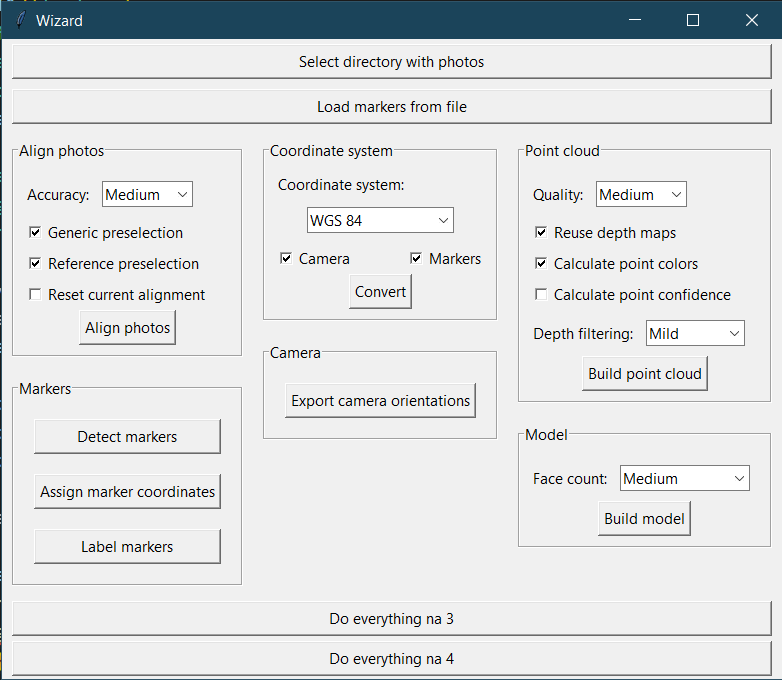
\includegraphics[width=0.75\textwidth]{img/interfejs.png}
    \caption*{}
\end{figure}

\section{Instrukcja obsługi}
\subsection{Zadanie 3.0}
Po uruchomieniu programu należy wcisnąć przycisk \textit{Select directory with photos}. Po kliknięciu przycisku zostanie najpierw uruchomione okno pozwalające na wybór układu współrzędnych, w jakim mają zostać wczytane zdjęcia, a następnie okno pozwalające na wybór folderu ze zdjęciami.
Następnie należy dostosować ustawienia dotyczące wyrównania zdjęć, układu współrzędnych, chmury punktów oraz modelu. Po dostosowaniu wszystkich opcji należy wcisnąć przycisk \textit{Do everything na 3}.
Efektem działania programu jest wyrównanie zdjęć, w zależności od wyboru opcji konwersja kamer i markerów do odpowiedniego układu współrzędnych, a także utworzenie chmury punktów oraz modelu. Chmura punktów oraz model zostają zapisane w folderze zawierającym zdjęcia.

\subsection{Zadanie 4.0}
Po uruchomieniu programu należy wcisnąć przycisk \textit{Select directory with photos}. Po kliknięciu przycisku zostanie najpierw uruchomione okno pozwalające na wybór układu współrzędnych, w jakim mają zostać wczytane zdjęcia, a następnie okno pozwalające na wybór folderu ze zdjęciami.

Następnie należy wczytać markery za pomocą przycisku \textit{Load markers from file}. Po kliknięciu przycisku zostanie najpierw uruchomione okno pozwalające na wybór układu współrzędnych, w jakim zapisane są markery w pliku, a następnie okno pozwalające na wybór pliku txt z markerami. Za pomocą przycisku \textit{Align photos} po wyborze ustawień należy wyrównać zdjęcia. Następnie należy pomierzyć manualnie kilka markerów na kilku zdjęciach. Po wykonaniu działań należy wcisnąć przycisk \textit{Do everything na 4}.

Program odświeża układ po pomierzeniu markerów, następnie automatycznie wykrywa markery krzyżowe ze zdjęć za pomocą chunk.detectMarkers(Metashape.TargetType.CrossTarget). Automatycznie przypisuje im współrzędne, a później po odnalezieniu odpowiadającego mu markera z pliku txt dodaje mu odpowiedni label.

Program eksportuje elementy orientacji zewnętrznej zdjęć do pliku tekstowego w folderze ze zdjęciami.

\end{document}